\documentclass[1p]{elsarticle_modified}
%\bibliographystyle{elsarticle-num}

%\usepackage[colorlinks]{hyperref}
%\usepackage{abbrmath_seonhwa} %\Abb, \Ascr, \Acal ,\Abf, \Afrak
\usepackage{amsfonts}
\usepackage{amssymb}
\usepackage{amsmath}
\usepackage{amsthm}
\usepackage{scalefnt}
\usepackage{amsbsy}
\usepackage{kotex}
\usepackage{caption}
\usepackage{subfig}
\usepackage{color}
\usepackage{graphicx}
\usepackage{xcolor} %% white, black, red, green, blue, cyan, magenta, yellow
\usepackage{float}
\usepackage{setspace}
\usepackage{hyperref}

\usepackage{tikz}
\usetikzlibrary{arrows}

\usepackage{multirow}
\usepackage{array} % fixed length table
\usepackage{hhline}

%%%%%%%%%%%%%%%%%%%%%
\makeatletter
\renewcommand*\env@matrix[1][\arraystretch]{%
	\edef\arraystretch{#1}%
	\hskip -\arraycolsep
	\let\@ifnextchar\new@ifnextchar
	\array{*\c@MaxMatrixCols c}}
\makeatother %https://tex.stackexchange.com/questions/14071/how-can-i-increase-the-line-spacing-in-a-matrix
%%%%%%%%%%%%%%%

\usepackage[normalem]{ulem}

\newcommand{\msout}[1]{\ifmmode\text{\sout{\ensuremath{#1}}}\else\sout{#1}\fi}
%SOURCE: \msout is \stkout macro in https://tex.stackexchange.com/questions/20609/strikeout-in-math-mode

\newcommand{\cancel}[1]{
	\ifmmode
	{\color{red}\msout{#1}}
	\else
	{\color{red}\sout{#1}}
	\fi
}

\newcommand{\add}[1]{
	{\color{blue}\uwave{#1}}
}

\newcommand{\replace}[2]{
	\ifmmode
	{\color{red}\msout{#1}}{\color{blue}\uwave{#2}}
	\else
	{\color{red}\sout{#1}}{\color{blue}\uwave{#2}}
	\fi
}

\newcommand{\Sol}{\mathcal{S}} %segment
\newcommand{\D}{D} %diagram
\newcommand{\A}{\mathcal{A}} %arc


%%%%%%%%%%%%%%%%%%%%%%%%%%%%%5 test

\def\sl{\operatorname{\textup{SL}}(2,\Cbb)}
\def\psl{\operatorname{\textup{PSL}}(2,\Cbb)}
\def\quan{\mkern 1mu \triangleright \mkern 1mu}

\theoremstyle{definition}
\newtheorem{thm}{Theorem}[section]
\newtheorem{prop}[thm]{Proposition}
\newtheorem{lem}[thm]{Lemma}
\newtheorem{ques}[thm]{Question}
\newtheorem{cor}[thm]{Corollary}
\newtheorem{defn}[thm]{Definition}
\newtheorem{exam}[thm]{Example}
\newtheorem{rmk}[thm]{Remark}
\newtheorem{alg}[thm]{Algorithm}

\newcommand{\I}{\sqrt{-1}}
\begin{document}

%\begin{frontmatter}
%
%\title{Boundary parabolic representations of knots up to 8 crossings}
%
%%% Group authors per affiliation:
%\author{Yunhi Cho} 
%\address{Department of Mathematics, University of Seoul, Seoul, Korea}
%\ead{yhcho@uos.ac.kr}
%
%
%\author{Seonhwa Kim} %\fnref{s_kim}}
%\address{Center for Geometry and Physics, Institute for Basic Science, Pohang, 37673, Korea}
%\ead{ryeona17@ibs.re.kr}
%
%\author{Hyuk Kim}
%\address{Department of Mathematical Sciences, Seoul National University, Seoul 08826, Korea}
%\ead{hyukkim@snu.ac.kr}
%
%\author{Seokbeom Yoon}
%\address{Department of Mathematical Sciences, Seoul National University, Seoul, 08826,  Korea}
%\ead{sbyoon15@snu.ac.kr}
%
%\begin{abstract}
%We find all boundary parabolic representation of knots up to 8 crossings.
%
%\end{abstract}
%\begin{keyword}
%    \MSC[2010] 57M25 
%\end{keyword}
%
%\end{frontmatter}

%\linenumbers
%\tableofcontents
%
\newcommand\colored[1]{\textcolor{white}{\rule[-0.35ex]{0.8em}{1.4ex}}\kern-0.8em\color{red} #1}%
%\newcommand\colored[1]{\textcolor{white}{ #1}\kern-2.17ex	\textcolor{white}{ #1}\kern-1.81ex	\textcolor{white}{ #1}\kern-2.15ex\color{red}#1	}

{\Large $\underline{12a_{0171}~(K12a_{0171})}$}

\setlength{\tabcolsep}{10pt}
\renewcommand{\arraystretch}{1.6}
\vspace{1cm}\begin{tabular}{m{100pt}>{\centering\arraybackslash}m{274pt}}
\multirow{5}{120pt}{
	\centering
	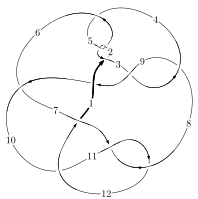
\includegraphics[width=112pt]{../../../GIT/diagram.site/Diagrams/png/972_12a_0171.png}\\
\ \ \ A knot diagram\footnotemark}&
\allowdisplaybreaks
\textbf{Linearized knot diagam} \\
\cline{2-2}
 &
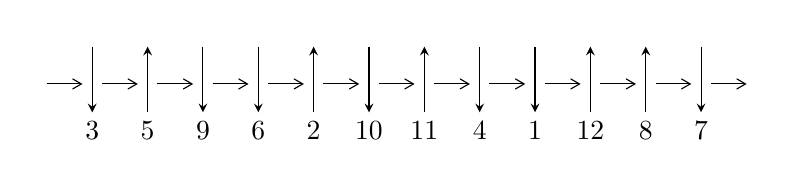
\begin{tikzpicture}[x=20pt, y=17pt]
	% nodes
	\node (C0) at (0, 0) {};
	\node (C1) at (1, 0) {};
	\node (C1U) at (1, +1) {};
	\node (C1D) at (1, -1) {3};

	\node (C2) at (2, 0) {};
	\node (C2U) at (2, +1) {};
	\node (C2D) at (2, -1) {5};

	\node (C3) at (3, 0) {};
	\node (C3U) at (3, +1) {};
	\node (C3D) at (3, -1) {9};

	\node (C4) at (4, 0) {};
	\node (C4U) at (4, +1) {};
	\node (C4D) at (4, -1) {6};

	\node (C5) at (5, 0) {};
	\node (C5U) at (5, +1) {};
	\node (C5D) at (5, -1) {2};

	\node (C6) at (6, 0) {};
	\node (C6U) at (6, +1) {};
	\node (C6D) at (6, -1) {10};

	\node (C7) at (7, 0) {};
	\node (C7U) at (7, +1) {};
	\node (C7D) at (7, -1) {11};

	\node (C8) at (8, 0) {};
	\node (C8U) at (8, +1) {};
	\node (C8D) at (8, -1) {4};

	\node (C9) at (9, 0) {};
	\node (C9U) at (9, +1) {};
	\node (C9D) at (9, -1) {1};

	\node (C10) at (10, 0) {};
	\node (C10U) at (10, +1) {};
	\node (C10D) at (10, -1) {12};

	\node (C11) at (11, 0) {};
	\node (C11U) at (11, +1) {};
	\node (C11D) at (11, -1) {8};

	\node (C12) at (12, 0) {};
	\node (C12U) at (12, +1) {};
	\node (C12D) at (12, -1) {7};
	\node (C13) at (13, 0) {};

	% arrows
	\draw[->,>={angle 60}]
	(C0) edge (C1) (C1) edge (C2) (C2) edge (C3) (C3) edge (C4) (C4) edge (C5) (C5) edge (C6) (C6) edge (C7) (C7) edge (C8) (C8) edge (C9) (C9) edge (C10) (C10) edge (C11) (C11) edge (C12) (C12) edge (C13) ;	\draw[->,>=stealth]
	(C1U) edge (C1D) (C2D) edge (C2U) (C3U) edge (C3D) (C4U) edge (C4D) (C5D) edge (C5U) (C6U) edge (C6D) (C7D) edge (C7U) (C8U) edge (C8D) (C9U) edge (C9D) (C10D) edge (C10U) (C11D) edge (C11U) (C12U) edge (C12D) ;
	\end{tikzpicture} \\
\hhline{~~} \\& 
\textbf{Solving Sequence} \\ \cline{2-2} 
 &
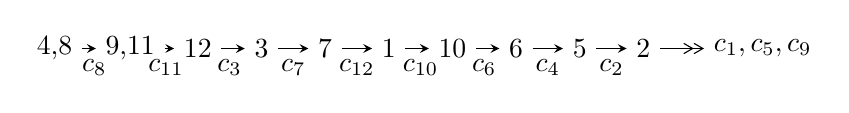
\begin{tikzpicture}[x=23pt, y=7pt]
	% node
	\node (A0) at (-1/8, 0) {4,8};
	\node (A1) at (17/16, 0) {9,11};
	\node (A2) at (17/8, 0) {12};
	\node (A3) at (25/8, 0) {3};
	\node (A4) at (33/8, 0) {7};
	\node (A5) at (41/8, 0) {1};
	\node (A6) at (49/8, 0) {10};
	\node (A7) at (57/8, 0) {6};
	\node (A8) at (65/8, 0) {5};
	\node (A9) at (73/8, 0) {2};
	\node (C1) at (1/2, -1) {$c_{8}$};
	\node (C2) at (13/8, -1) {$c_{11}$};
	\node (C3) at (21/8, -1) {$c_{3}$};
	\node (C4) at (29/8, -1) {$c_{7}$};
	\node (C5) at (37/8, -1) {$c_{12}$};
	\node (C6) at (45/8, -1) {$c_{10}$};
	\node (C7) at (53/8, -1) {$c_{6}$};
	\node (C8) at (61/8, -1) {$c_{4}$};
	\node (C9) at (69/8, -1) {$c_{2}$};
	\node (A10) at (11, 0) {$c_{1},c_{5},c_{9}$};

	% edge
	\draw[->,>=stealth]	
	(A0) edge (A1) (A1) edge (A2) (A2) edge (A3) (A3) edge (A4) (A4) edge (A5) (A5) edge (A6) (A6) edge (A7) (A7) edge (A8) (A8) edge (A9) ;
	\draw[->>,>={angle 60}]	
	(A9) edge (A10);
\end{tikzpicture} \\ 

\end{tabular} \\

\footnotetext{
The image of knot diagram is generated by the software ``\textbf{Draw programme}" developed by Andrew Bartholomew(\url{http://www.layer8.co.uk/maths/draw/index.htm\#Running-draw}), where we modified some parts for our purpose(\url{https://github.com/CATsTAILs/LinksPainter}).
}\phantom \\ \newline 
\centering \textbf{Ideals for irreducible components\footnotemark of $X_{\text{par}}$} 
 
\begin{align*}
I^u_{1}&=\langle 
1.15819\times10^{360} u^{109}-4.02996\times10^{360} u^{108}+\cdots+5.49965\times10^{360} b-1.34535\times10^{364},\\
\phantom{I^u_{1}}&\phantom{= \langle  }-1.86842\times10^{361} u^{109}+2.18094\times10^{361} u^{108}+\cdots+1.09993\times10^{361} a+8.84584\times10^{363},\\
\phantom{I^u_{1}}&\phantom{= \langle  }u^{110}- u^{109}+\cdots-8192 u+4096\rangle \\
\\
I^v_{1}&=\langle 
a,\;v^3+b-1,\;v^{12}- v^{11}+v^{10}-4 v^9+3 v^8-3 v^7+5 v^6-3 v^5+3 v^4-3 v^3+2 v^2- v+1\rangle \\
\end{align*}
\raggedright * 2 irreducible components of $\dim_{\mathbb{C}}=0$, with total 122 representations.\\
\footnotetext{All coefficients of polynomials are rational numbers. But the coefficients are sometimes approximated in decimal forms when there is not enough margin.}
\newpage
\renewcommand{\arraystretch}{1}
\centering \section*{I. $I^u_{1}= \langle 1.16\times10^{360} u^{109}-4.03\times10^{360} u^{108}+\cdots+5.50\times10^{360} b-1.35\times10^{364},\;-1.87\times10^{361} u^{109}+2.18\times10^{361} u^{108}+\cdots+1.10\times10^{361} a+8.85\times10^{363},\;u^{110}- u^{109}+\cdots-8192 u+4096 \rangle$}
\flushleft \textbf{(i) Arc colorings}\\
\begin{tabular}{m{7pt} m{180pt} m{7pt} m{180pt} }
\flushright $a_{4}=$&$\begin{pmatrix}0\\u\end{pmatrix}$ \\
\flushright $a_{8}=$&$\begin{pmatrix}1\\0\end{pmatrix}$ \\
\flushright $a_{9}=$&$\begin{pmatrix}1\\u^2\end{pmatrix}$ \\
\flushright $a_{11}=$&$\begin{pmatrix}1.69867 u^{109}-1.98280 u^{108}+\cdots+9457.21 u-804.218\\-0.210593 u^{109}+0.732766 u^{108}+\cdots-5987.35 u+2446.24\end{pmatrix}$ \\
\flushright $a_{12}=$&$\begin{pmatrix}1.48808 u^{109}-1.25003 u^{108}+\cdots+3469.86 u+1642.02\\-0.210593 u^{109}+0.732766 u^{108}+\cdots-5987.35 u+2446.24\end{pmatrix}$ \\
\flushright $a_{3}=$&$\begin{pmatrix}u\\u^3+u\end{pmatrix}$ \\
\flushright $a_{7}=$&$\begin{pmatrix}0.714770 u^{109}-1.52578 u^{108}+\cdots+10789.3 u-3614.64\\0.337885 u^{109}+0.284437 u^{108}+\cdots-4404.48 u+2959.35\end{pmatrix}$ \\
\flushright $a_{1}=$&$\begin{pmatrix}1.13580 u^{109}-2.01555 u^{108}+\cdots+13081.2 u-3731.32\\1.06260 u^{109}-1.34601 u^{108}+\cdots+6511.41 u-918.245\end{pmatrix}$ \\
\flushright $a_{10}=$&$\begin{pmatrix}0.431583 u^{109}-0.532966 u^{108}+\cdots+2172.28 u-59.0907\\-0.724304 u^{109}+0.723872 u^{108}+\cdots-3494.65 u+30.9050\end{pmatrix}$ \\
\flushright $a_{6}=$&$\begin{pmatrix}-0.857528 u^{109}+1.09821 u^{108}+\cdots-5289.40 u+790.397\\-1.99332 u^{109}+3.11376 u^{108}+\cdots-18370.6 u+4521.72\end{pmatrix}$ \\
\flushright $a_{5}=$&$\begin{pmatrix}0.00285440 u^{109}+0.527936 u^{108}+\cdots-5539.52 u+2531.27\\0.0673513 u^{109}-0.758670 u^{108}+\cdots+6801.27 u-3238.00\end{pmatrix}$ \\
\flushright $a_{2}=$&$\begin{pmatrix}1.93960 u^{109}-3.10158 u^{108}+\cdots+18565.3 u-4717.17\\1.11994 u^{109}-1.36855 u^{108}+\cdots+6391.16 u-748.098\end{pmatrix}$\\&\end{tabular}
\flushleft \textbf{(ii) Obstruction class $= -1$}\\~\\
\flushleft \textbf{(iii) Cusp Shapes $= -2.48768 u^{109}+4.72242 u^{108}+\cdots-31628.9 u+9674.98$}\\~\\
\newpage\renewcommand{\arraystretch}{1}
\flushleft \textbf{(iv) u-Polynomials at the component}\newline \\
\begin{tabular}{m{50pt}|m{274pt}}
Crossings & \hspace{64pt}u-Polynomials at each crossing \\
\hline $$\begin{aligned}c_{1},c_{4}\end{aligned}$$&$\begin{aligned}
&u^{110}+35 u^{109}+\cdots+3 u+1
\end{aligned}$\\
\hline $$\begin{aligned}c_{2},c_{5}\end{aligned}$$&$\begin{aligned}
&u^{110}+7 u^{109}+\cdots+7 u+1
\end{aligned}$\\
\hline $$\begin{aligned}c_{3},c_{8}\end{aligned}$$&$\begin{aligned}
&u^{110}+u^{109}+\cdots+8192 u+4096
\end{aligned}$\\
\hline $$\begin{aligned}c_{6}\end{aligned}$$&$\begin{aligned}
&u^{110}+3 u^{109}+\cdots+1599 u+1297
\end{aligned}$\\
\hline $$\begin{aligned}c_{7},c_{11}\end{aligned}$$&$\begin{aligned}
&u^{110}-3 u^{109}+\cdots-5 u+1
\end{aligned}$\\
\hline $$\begin{aligned}c_{9}\end{aligned}$$&$\begin{aligned}
&u^{110}-11 u^{109}+\cdots-299803 u+6701
\end{aligned}$\\
\hline $$\begin{aligned}c_{10}\end{aligned}$$&$\begin{aligned}
&u^{110}-53 u^{109}+\cdots+7 u+1
\end{aligned}$\\
\hline $$\begin{aligned}c_{12}\end{aligned}$$&$\begin{aligned}
&u^{110}-9 u^{109}+\cdots+6069 u+851
\end{aligned}$\\
\hline
\end{tabular}\\~\\
\newpage\renewcommand{\arraystretch}{1}
\flushleft \textbf{(v) Riley Polynomials at the component}\newline \\
\begin{tabular}{m{50pt}|m{274pt}}
Crossings & \hspace{64pt}Riley Polynomials at each crossing \\
\hline $$\begin{aligned}c_{1},c_{4}\end{aligned}$$&$\begin{aligned}
&y^{110}+87 y^{109}+\cdots-9 y+1
\end{aligned}$\\
\hline $$\begin{aligned}c_{2},c_{5}\end{aligned}$$&$\begin{aligned}
&y^{110}+35 y^{109}+\cdots+3 y+1
\end{aligned}$\\
\hline $$\begin{aligned}c_{3},c_{8}\end{aligned}$$&$\begin{aligned}
&y^{110}+65 y^{109}+\cdots+268435456 y+16777216
\end{aligned}$\\
\hline $$\begin{aligned}c_{6}\end{aligned}$$&$\begin{aligned}
&y^{110}-13 y^{109}+\cdots-35448721 y+1682209
\end{aligned}$\\
\hline $$\begin{aligned}c_{7},c_{11}\end{aligned}$$&$\begin{aligned}
&y^{110}-53 y^{109}+\cdots+7 y+1
\end{aligned}$\\
\hline $$\begin{aligned}c_{9}\end{aligned}$$&$\begin{aligned}
&y^{110}+47 y^{109}+\cdots+20676298343 y+44903401
\end{aligned}$\\
\hline $$\begin{aligned}c_{10}\end{aligned}$$&$\begin{aligned}
&y^{110}+11 y^{109}+\cdots-49 y+1
\end{aligned}$\\
\hline $$\begin{aligned}c_{12}\end{aligned}$$&$\begin{aligned}
&y^{110}+31 y^{109}+\cdots-29575433 y+724201
\end{aligned}$\\
\hline
\end{tabular}\\~\\
\newpage\flushleft \textbf{(vi) Complex Volumes and Cusp Shapes}
$$\begin{array}{c|c|c}  
\text{Solutions to }I^u_{1}& \I (\text{vol} + \sqrt{-1}CS) & \text{Cusp shape}\\
 \hline 
\begin{aligned}
u &= -0.180529 + 0.981799 I \\
a &= \phantom{-}0.436047 - 0.614290 I \\
b &= \phantom{-}0.491906 - 0.727885 I\end{aligned}
 & -0.53209 + 3.96936 I & \phantom{-0.000000 } 0 \\ \hline\begin{aligned}
u &= -0.180529 - 0.981799 I \\
a &= \phantom{-}0.436047 + 0.614290 I \\
b &= \phantom{-}0.491906 + 0.727885 I\end{aligned}
 & -0.53209 - 3.96936 I & \phantom{-0.000000 } 0 \\ \hline\begin{aligned}
u &= -0.957729 + 0.306652 I \\
a &= \phantom{-}0.696769 - 0.934630 I \\
b &= \phantom{-}0.640335 - 0.557300 I\end{aligned}
 & -0.05454 - 4.42932 I & \phantom{-0.000000 } 0 \\ \hline\begin{aligned}
u &= -0.957729 - 0.306652 I \\
a &= \phantom{-}0.696769 + 0.934630 I \\
b &= \phantom{-}0.640335 + 0.557300 I\end{aligned}
 & -0.05454 + 4.42932 I & \phantom{-0.000000 } 0 \\ \hline\begin{aligned}
u &= \phantom{-}0.245291 + 0.984450 I \\
a &= -0.56407 - 1.41967 I \\
b &= \phantom{-}1.049850 - 0.596683 I\end{aligned}
 & \phantom{-}1.11589 - 9.02457 I & \phantom{-0.000000 } 0 \\ \hline\begin{aligned}
u &= \phantom{-}0.245291 - 0.984450 I \\
a &= -0.56407 + 1.41967 I \\
b &= \phantom{-}1.049850 + 0.596683 I\end{aligned}
 & \phantom{-}1.11589 + 9.02457 I & \phantom{-0.000000 } 0 \\ \hline\begin{aligned}
u &= \phantom{-}0.532933 + 0.873851 I \\
a &= \phantom{-}0.084707 + 0.191205 I \\
b &= -0.954325 - 0.534058 I\end{aligned}
 & -2.00995 + 0.05811 I & \phantom{-0.000000 } 0 \\ \hline\begin{aligned}
u &= \phantom{-}0.532933 - 0.873851 I \\
a &= \phantom{-}0.084707 - 0.191205 I \\
b &= -0.954325 + 0.534058 I\end{aligned}
 & -2.00995 - 0.05811 I & \phantom{-0.000000 } 0 \\ \hline\begin{aligned}
u &= -0.105007 + 1.018520 I \\
a &= -3.29953 - 0.20001 I \\
b &= \phantom{-}1.108910 + 0.314775 I\end{aligned}
 & \phantom{-}3.39141 + 3.62653 I & \phantom{-0.000000 } 0 \\ \hline\begin{aligned}
u &= -0.105007 - 1.018520 I \\
a &= -3.29953 + 0.20001 I \\
b &= \phantom{-}1.108910 - 0.314775 I\end{aligned}
 & \phantom{-}3.39141 - 3.62653 I & \phantom{-0.000000 } 0\\
 \hline 
 \end{array}$$\newpage$$\begin{array}{c|c|c}  
\text{Solutions to }I^u_{1}& \I (\text{vol} + \sqrt{-1}CS) & \text{Cusp shape}\\
 \hline 
\begin{aligned}
u &= \phantom{-}0.059861 + 1.025080 I \\
a &= \phantom{-}3.21011 + 0.60441 I \\
b &= -1.114020 + 0.535031 I\end{aligned}
 & \phantom{-}1.88520 - 3.91301 I & \phantom{-0.000000 } 0 \\ \hline\begin{aligned}
u &= \phantom{-}0.059861 - 1.025080 I \\
a &= \phantom{-}3.21011 - 0.60441 I \\
b &= -1.114020 - 0.535031 I\end{aligned}
 & \phantom{-}1.88520 + 3.91301 I & \phantom{-0.000000 } 0 \\ \hline\begin{aligned}
u &= \phantom{-}0.196284 + 0.944858 I \\
a &= \phantom{-}0.947750 + 0.572093 I \\
b &= -0.665914 + 0.514784 I\end{aligned}
 & \phantom{-}0.83286 - 1.92222 I & \phantom{-0.000000 } 0 \\ \hline\begin{aligned}
u &= \phantom{-}0.196284 - 0.944858 I \\
a &= \phantom{-}0.947750 - 0.572093 I \\
b &= -0.665914 - 0.514784 I\end{aligned}
 & \phantom{-}0.83286 + 1.92222 I & \phantom{-0.000000 } 0 \\ \hline\begin{aligned}
u &= -0.042659 + 0.963890 I \\
a &= \phantom{-}0.429644 + 0.579531 I \\
b &= \phantom{-}0.466727 + 0.736300 I\end{aligned}
 & -0.40492 + 1.37362 I & \phantom{-0.000000 } 0 \\ \hline\begin{aligned}
u &= -0.042659 - 0.963890 I \\
a &= \phantom{-}0.429644 - 0.579531 I \\
b &= \phantom{-}0.466727 - 0.736300 I\end{aligned}
 & -0.40492 - 1.37362 I & \phantom{-0.000000 } 0 \\ \hline\begin{aligned}
u &= -0.020984 + 0.946768 I \\
a &= -0.62326 + 1.38833 I \\
b &= \phantom{-}1.065210 + 0.594026 I\end{aligned}
 & \phantom{-}1.36280 + 3.69257 I & \phantom{-0.000000 } 0 \\ \hline\begin{aligned}
u &= -0.020984 - 0.946768 I \\
a &= -0.62326 - 1.38833 I \\
b &= \phantom{-}1.065210 - 0.594026 I\end{aligned}
 & \phantom{-}1.36280 - 3.69257 I & \phantom{-0.000000 } 0 \\ \hline\begin{aligned}
u &= -0.045031 + 0.927975 I \\
a &= \phantom{-}0.019136 - 1.251560 I \\
b &= -0.294206 + 0.667943 I\end{aligned}
 & -0.456573 - 0.751770 I & \phantom{-0.000000 } 0 \\ \hline\begin{aligned}
u &= -0.045031 - 0.927975 I \\
a &= \phantom{-}0.019136 + 1.251560 I \\
b &= -0.294206 - 0.667943 I\end{aligned}
 & -0.456573 + 0.751770 I & \phantom{-0.000000 } 0\\
 \hline 
 \end{array}$$\newpage$$\begin{array}{c|c|c}  
\text{Solutions to }I^u_{1}& \I (\text{vol} + \sqrt{-1}CS) & \text{Cusp shape}\\
 \hline 
\begin{aligned}
u &= -0.490706 + 0.956042 I \\
a &= \phantom{-}0.90556 - 1.10461 I \\
b &= -0.616458 - 0.613746 I\end{aligned}
 & -2.99794 + 4.49260 I & \phantom{-0.000000 } 0 \\ \hline\begin{aligned}
u &= -0.490706 - 0.956042 I \\
a &= \phantom{-}0.90556 + 1.10461 I \\
b &= -0.616458 + 0.613746 I\end{aligned}
 & -2.99794 - 4.49260 I & \phantom{-0.000000 } 0 \\ \hline\begin{aligned}
u &= \phantom{-}0.649259 + 0.651850 I \\
a &= -0.49900 - 1.69164 I \\
b &= \phantom{-}1.012510 - 0.555888 I\end{aligned}
 & -2.73974 - 4.65409 I & \phantom{-0.000000 } 0 \\ \hline\begin{aligned}
u &= \phantom{-}0.649259 - 0.651850 I \\
a &= -0.49900 + 1.69164 I \\
b &= \phantom{-}1.012510 + 0.555888 I\end{aligned}
 & -2.73974 + 4.65409 I & \phantom{-0.000000 } 0 \\ \hline\begin{aligned}
u &= -0.641134 + 0.595733 I \\
a &= \phantom{-}0.551507 - 0.699489 I \\
b &= \phantom{-}0.536320 - 0.644113 I\end{aligned}
 & -4.14246 - 0.04555 I & \phantom{-0.000000 } 0 \\ \hline\begin{aligned}
u &= -0.641134 - 0.595733 I \\
a &= \phantom{-}0.551507 + 0.699489 I \\
b &= \phantom{-}0.536320 + 0.644113 I\end{aligned}
 & -4.14246 + 0.04555 I & \phantom{-0.000000 } 0 \\ \hline\begin{aligned}
u &= -0.725461 + 0.479876 I \\
a &= -1.02784 + 2.23874 I \\
b &= \phantom{-}1.031940 + 0.469288 I\end{aligned}
 & \phantom{-}1.74989 + 4.60006 I & \phantom{-0.000000 } 0 \\ \hline\begin{aligned}
u &= -0.725461 - 0.479876 I \\
a &= -1.02784 - 2.23874 I \\
b &= \phantom{-}1.031940 - 0.469288 I\end{aligned}
 & \phantom{-}1.74989 - 4.60006 I & \phantom{-0.000000 } 0 \\ \hline\begin{aligned}
u &= \phantom{-}0.085944 + 1.128550 I \\
a &= \phantom{-}0.999975 + 0.000279 I \\
b &= -1.045510 + 0.024442 I\end{aligned}
 & \phantom{-}4.66020 - 2.81279 I & \phantom{-0.000000 } 0 \\ \hline\begin{aligned}
u &= \phantom{-}0.085944 - 1.128550 I \\
a &= \phantom{-}0.999975 - 0.000279 I \\
b &= -1.045510 - 0.024442 I\end{aligned}
 & \phantom{-}4.66020 + 2.81279 I & \phantom{-0.000000 } 0\\
 \hline 
 \end{array}$$\newpage$$\begin{array}{c|c|c}  
\text{Solutions to }I^u_{1}& \I (\text{vol} + \sqrt{-1}CS) & \text{Cusp shape}\\
 \hline 
\begin{aligned}
u &= \phantom{-}0.845787 + 0.182009 I \\
a &= \phantom{-}0.934137 + 0.898042 I \\
b &= \phantom{-}0.627147 + 0.468257 I\end{aligned}
 & \phantom{-}0.388388 - 0.807655 I & \phantom{-0.000000 } 0 \\ \hline\begin{aligned}
u &= \phantom{-}0.845787 - 0.182009 I \\
a &= \phantom{-}0.934137 - 0.898042 I \\
b &= \phantom{-}0.627147 - 0.468257 I\end{aligned}
 & \phantom{-}0.388388 + 0.807655 I & \phantom{-0.000000 } 0 \\ \hline\begin{aligned}
u &= \phantom{-}1.130550 + 0.136437 I \\
a &= \phantom{-}0.448643 - 0.344341 I \\
b &= \phantom{-}0.278130 - 0.714398 I\end{aligned}
 & \phantom{-}1.86533 + 0.28927 I & \phantom{-0.000000 } 0 \\ \hline\begin{aligned}
u &= \phantom{-}1.130550 - 0.136437 I \\
a &= \phantom{-}0.448643 + 0.344341 I \\
b &= \phantom{-}0.278130 + 0.714398 I\end{aligned}
 & \phantom{-}1.86533 - 0.28927 I & \phantom{-0.000000 } 0 \\ \hline\begin{aligned}
u &= \phantom{-}0.748053 + 0.425580 I \\
a &= -0.32882 - 2.51211 I \\
b &= \phantom{-}0.972826 - 0.468613 I\end{aligned}
 & \phantom{-}0.873774 + 0.295236 I & \phantom{-0.000000 } 0 \\ \hline\begin{aligned}
u &= \phantom{-}0.748053 - 0.425580 I \\
a &= -0.32882 + 2.51211 I \\
b &= \phantom{-}0.972826 + 0.468613 I\end{aligned}
 & \phantom{-}0.873774 - 0.295236 I & \phantom{-0.000000 } 0 \\ \hline\begin{aligned}
u &= \phantom{-}0.368685 + 1.078770 I \\
a &= -2.18116 - 1.37265 I \\
b &= \phantom{-}1.120270 + 0.256088 I\end{aligned}
 & \phantom{-}2.76276 - 3.58996 I & \phantom{-0.000000 } 0 \\ \hline\begin{aligned}
u &= \phantom{-}0.368685 - 1.078770 I \\
a &= -2.18116 + 1.37265 I \\
b &= \phantom{-}1.120270 - 0.256088 I\end{aligned}
 & \phantom{-}2.76276 + 3.58996 I & \phantom{-0.000000 } 0 \\ \hline\begin{aligned}
u &= -0.484397 + 0.700403 I \\
a &= \phantom{-}0.939042 - 0.555934 I \\
b &= -1.023720 + 0.450046 I\end{aligned}
 & \phantom{-}1.87514 - 1.78615 I & \phantom{-0.000000 } 0 \\ \hline\begin{aligned}
u &= -0.484397 - 0.700403 I \\
a &= \phantom{-}0.939042 + 0.555934 I \\
b &= -1.023720 - 0.450046 I\end{aligned}
 & \phantom{-}1.87514 + 1.78615 I & \phantom{-0.000000 } 0\\
 \hline 
 \end{array}$$\newpage$$\begin{array}{c|c|c}  
\text{Solutions to }I^u_{1}& \I (\text{vol} + \sqrt{-1}CS) & \text{Cusp shape}\\
 \hline 
\begin{aligned}
u &= -0.450007 + 1.072020 I \\
a &= -0.871246 - 0.709105 I \\
b &= -0.323796 + 0.743902 I\end{aligned}
 & -1.61375 + 6.35314 I & \phantom{-0.000000 } 0 \\ \hline\begin{aligned}
u &= -0.450007 - 1.072020 I \\
a &= -0.871246 + 0.709105 I \\
b &= -0.323796 - 0.743902 I\end{aligned}
 & -1.61375 - 6.35314 I & \phantom{-0.000000 } 0 \\ \hline\begin{aligned}
u &= \phantom{-}0.465125 + 0.693500 I \\
a &= \phantom{-}0.54861 + 1.38506 I \\
b &= -1.032120 - 0.509724 I\end{aligned}
 & \phantom{-}0.29498 + 6.14668 I & \phantom{-0.000000 } 0 \\ \hline\begin{aligned}
u &= \phantom{-}0.465125 - 0.693500 I \\
a &= \phantom{-}0.54861 - 1.38506 I \\
b &= -1.032120 + 0.509724 I\end{aligned}
 & \phantom{-}0.29498 - 6.14668 I & \phantom{-0.000000 } 0 \\ \hline\begin{aligned}
u &= -0.636626 + 0.511266 I \\
a &= \phantom{-}0.458277 + 0.471434 I \\
b &= \phantom{-}0.381330 + 0.717360 I\end{aligned}
 & -3.40779 - 2.06523 I & \phantom{-0.000000 } 0 \\ \hline\begin{aligned}
u &= -0.636626 - 0.511266 I \\
a &= \phantom{-}0.458277 - 0.471434 I \\
b &= \phantom{-}0.381330 - 0.717360 I\end{aligned}
 & -3.40779 + 2.06523 I & \phantom{-0.000000 } 0 \\ \hline\begin{aligned}
u &= -1.184690 + 0.040759 I \\
a &= \phantom{-}1.096850 + 0.011640 I \\
b &= -1.129150 - 0.296830 I\end{aligned}
 & \phantom{-}5.96201 + 2.70522 I & \phantom{-0.000000 } 0 \\ \hline\begin{aligned}
u &= -1.184690 - 0.040759 I \\
a &= \phantom{-}1.096850 - 0.011640 I \\
b &= -1.129150 + 0.296830 I\end{aligned}
 & \phantom{-}5.96201 - 2.70522 I & \phantom{-0.000000 } 0 \\ \hline\begin{aligned}
u &= -1.150850 + 0.292842 I \\
a &= \phantom{-}0.427388 + 0.371304 I \\
b &= \phantom{-}0.297385 + 0.735259 I\end{aligned}
 & \phantom{-}1.48990 - 5.94638 I & \phantom{-0.000000 } 0 \\ \hline\begin{aligned}
u &= -1.150850 - 0.292842 I \\
a &= \phantom{-}0.427388 - 0.371304 I \\
b &= \phantom{-}0.297385 - 0.735259 I\end{aligned}
 & \phantom{-}1.48990 + 5.94638 I & \phantom{-0.000000 } 0\\
 \hline 
 \end{array}$$\newpage$$\begin{array}{c|c|c}  
\text{Solutions to }I^u_{1}& \I (\text{vol} + \sqrt{-1}CS) & \text{Cusp shape}\\
 \hline 
\begin{aligned}
u &= \phantom{-}0.641277 + 0.481162 I \\
a &= -0.81379 + 1.36040 I \\
b &= \phantom{-}1.098180 + 0.566600 I\end{aligned}
 & -1.31118 + 6.97785 I & \phantom{-0.000000 } 0 \\ \hline\begin{aligned}
u &= \phantom{-}0.641277 - 0.481162 I \\
a &= -0.81379 - 1.36040 I \\
b &= \phantom{-}1.098180 - 0.566600 I\end{aligned}
 & -1.31118 - 6.97785 I & \phantom{-0.000000 } 0 \\ \hline\begin{aligned}
u &= \phantom{-}0.205359 + 1.181870 I \\
a &= -0.403773 + 0.734690 I \\
b &= -0.282394 - 0.729773 I\end{aligned}
 & \phantom{-}2.47472 - 3.21396 I & \phantom{-0.000000 } 0 \\ \hline\begin{aligned}
u &= \phantom{-}0.205359 - 1.181870 I \\
a &= -0.403773 - 0.734690 I \\
b &= -0.282394 + 0.729773 I\end{aligned}
 & \phantom{-}2.47472 + 3.21396 I & \phantom{-0.000000 } 0 \\ \hline\begin{aligned}
u &= \phantom{-}0.453466 + 1.111160 I \\
a &= \phantom{-}2.55908 + 1.80779 I \\
b &= -1.124140 + 0.559775 I\end{aligned}
 & \phantom{-}0.72608 - 11.29210 I & \phantom{-0.000000 } 0 \\ \hline\begin{aligned}
u &= \phantom{-}0.453466 - 1.111160 I \\
a &= \phantom{-}2.55908 - 1.80779 I \\
b &= -1.124140 - 0.559775 I\end{aligned}
 & \phantom{-}0.72608 + 11.29210 I & \phantom{-0.000000 } 0 \\ \hline\begin{aligned}
u &= -1.190690 + 0.160033 I \\
a &= -0.99139 - 1.29273 I \\
b &= \phantom{-}1.126970 - 0.540371 I\end{aligned}
 & \phantom{-}4.31167 - 5.06642 I & \phantom{-0.000000 } 0 \\ \hline\begin{aligned}
u &= -1.190690 - 0.160033 I \\
a &= -0.99139 + 1.29273 I \\
b &= \phantom{-}1.126970 + 0.540371 I\end{aligned}
 & \phantom{-}4.31167 + 5.06642 I & \phantom{-0.000000 } 0 \\ \hline\begin{aligned}
u &= \phantom{-}1.188990 + 0.206425 I \\
a &= \phantom{-}1.078590 - 0.003691 I \\
b &= -1.130880 + 0.277395 I\end{aligned}
 & \phantom{-}5.74865 + 3.02431 I & \phantom{-0.000000 } 0 \\ \hline\begin{aligned}
u &= \phantom{-}1.188990 - 0.206425 I \\
a &= \phantom{-}1.078590 + 0.003691 I \\
b &= -1.130880 - 0.277395 I\end{aligned}
 & \phantom{-}5.74865 - 3.02431 I & \phantom{-0.000000 } 0\\
 \hline 
 \end{array}$$\newpage$$\begin{array}{c|c|c}  
\text{Solutions to }I^u_{1}& \I (\text{vol} + \sqrt{-1}CS) & \text{Cusp shape}\\
 \hline 
\begin{aligned}
u &= -0.120046 + 1.229700 I \\
a &= -2.47515 + 0.66044 I \\
b &= \phantom{-}1.134800 - 0.287824 I\end{aligned}
 & \phantom{-}6.66882 + 0.21455 I & \phantom{-0.000000 } 0 \\ \hline\begin{aligned}
u &= -0.120046 - 1.229700 I \\
a &= -2.47515 - 0.66044 I \\
b &= \phantom{-}1.134800 + 0.287824 I\end{aligned}
 & \phantom{-}6.66882 - 0.21455 I & \phantom{-0.000000 } 0 \\ \hline\begin{aligned}
u &= \phantom{-}1.198980 + 0.310591 I \\
a &= -0.94829 + 1.26895 I \\
b &= \phantom{-}1.128520 + 0.550313 I\end{aligned}
 & \phantom{-}3.90634 + 10.81930 I & \phantom{-0.000000 } 0 \\ \hline\begin{aligned}
u &= \phantom{-}1.198980 - 0.310591 I \\
a &= -0.94829 - 1.26895 I \\
b &= \phantom{-}1.128520 - 0.550313 I\end{aligned}
 & \phantom{-}3.90634 - 10.81930 I & \phantom{-0.000000 } 0 \\ \hline\begin{aligned}
u &= \phantom{-}0.569124 + 0.493960 I \\
a &= \phantom{-}1.018900 - 0.025895 I \\
b &= -1.049650 + 0.227586 I\end{aligned}
 & \phantom{-}0.920628 - 0.155382 I & \phantom{-0.000000 } 0 \\ \hline\begin{aligned}
u &= \phantom{-}0.569124 - 0.493960 I \\
a &= \phantom{-}1.018900 + 0.025895 I \\
b &= -1.049650 - 0.227586 I\end{aligned}
 & \phantom{-}0.920628 + 0.155382 I & \phantom{-0.000000 } 0 \\ \hline\begin{aligned}
u &= -0.279474 + 0.697539 I \\
a &= \phantom{-}1.83135 - 0.50580 I \\
b &= -0.501982 - 0.530747 I\end{aligned}
 & -1.28186 - 1.88031 I & \phantom{-0.000000 } 0 \\ \hline\begin{aligned}
u &= -0.279474 - 0.697539 I \\
a &= \phantom{-}1.83135 + 0.50580 I \\
b &= -0.501982 + 0.530747 I\end{aligned}
 & -1.28186 + 1.88031 I & \phantom{-0.000000 } 0 \\ \hline\begin{aligned}
u &= -0.228922 + 1.233270 I \\
a &= \phantom{-}2.56564 - 1.13931 I \\
b &= -1.130270 - 0.544788 I\end{aligned}
 & \phantom{-}4.93107 + 8.04588 I & \phantom{-0.000000 } 0 \\ \hline\begin{aligned}
u &= -0.228922 - 1.233270 I \\
a &= \phantom{-}2.56564 + 1.13931 I \\
b &= -1.130270 + 0.544788 I\end{aligned}
 & \phantom{-}4.93107 - 8.04588 I & \phantom{-0.000000 } 0\\
 \hline 
 \end{array}$$\newpage$$\begin{array}{c|c|c}  
\text{Solutions to }I^u_{1}& \I (\text{vol} + \sqrt{-1}CS) & \text{Cusp shape}\\
 \hline 
\begin{aligned}
u &= -0.417717 + 1.241140 I \\
a &= \phantom{-}0.223034 + 0.351211 I \\
b &= -0.877035 + 0.586420 I\end{aligned}
 & \phantom{-}4.47958 - 0.57999 I & \phantom{-0.000000 } 0 \\ \hline\begin{aligned}
u &= -0.417717 - 1.241140 I \\
a &= \phantom{-}0.223034 - 0.351211 I \\
b &= -0.877035 - 0.586420 I\end{aligned}
 & \phantom{-}4.47958 + 0.57999 I & \phantom{-0.000000 } 0 \\ \hline\begin{aligned}
u &= \phantom{-}0.537463 + 1.234880 I \\
a &= \phantom{-}0.119374 - 0.342327 I \\
b &= -0.899213 - 0.595297 I\end{aligned}
 & \phantom{-}3.66551 - 5.28805 I & \phantom{-0.000000 } 0 \\ \hline\begin{aligned}
u &= \phantom{-}0.537463 - 1.234880 I \\
a &= \phantom{-}0.119374 + 0.342327 I \\
b &= -0.899213 + 0.595297 I\end{aligned}
 & \phantom{-}3.66551 + 5.28805 I & \phantom{-0.000000 } 0 \\ \hline\begin{aligned}
u &= \phantom{-}0.378428 + 0.509984 I \\
a &= \phantom{-}0.895553 - 0.098903 I \\
b &= -0.076718 + 0.345713 I\end{aligned}
 & -0.22364 - 1.43182 I & -1.59578 + 4.94774 I \\ \hline\begin{aligned}
u &= \phantom{-}0.378428 - 0.509984 I \\
a &= \phantom{-}0.895553 + 0.098903 I \\
b &= -0.076718 - 0.345713 I\end{aligned}
 & -0.22364 + 1.43182 I & -1.59578 - 4.94774 I \\ \hline\begin{aligned}
u &= \phantom{-}0.493923 + 1.274500 I \\
a &= \phantom{-}0.550307 + 0.943227 I \\
b &= -0.683310 + 0.649852 I\end{aligned}
 & \phantom{-}3.90406 - 4.23872 I & \phantom{-0.000000 } 0 \\ \hline\begin{aligned}
u &= \phantom{-}0.493923 - 1.274500 I \\
a &= \phantom{-}0.550307 - 0.943227 I \\
b &= -0.683310 - 0.649852 I\end{aligned}
 & \phantom{-}3.90406 + 4.23872 I & \phantom{-0.000000 } 0 \\ \hline\begin{aligned}
u &= -0.598872 + 0.202622 I \\
a &= -0.86845 + 1.56868 I \\
b &= \phantom{-}1.073350 + 0.535528 I\end{aligned}
 & \phantom{-}0.50426 + 5.26842 I & -1.42602 - 6.38867 I \\ \hline\begin{aligned}
u &= -0.598872 - 0.202622 I \\
a &= -0.86845 - 1.56868 I \\
b &= \phantom{-}1.073350 - 0.535528 I\end{aligned}
 & \phantom{-}0.50426 - 5.26842 I & -1.42602 + 6.38867 I\\
 \hline 
 \end{array}$$\newpage$$\begin{array}{c|c|c}  
\text{Solutions to }I^u_{1}& \I (\text{vol} + \sqrt{-1}CS) & \text{Cusp shape}\\
 \hline 
\begin{aligned}
u &= -0.593543 + 1.262890 I \\
a &= \phantom{-}0.520858 - 1.019690 I \\
b &= -0.670145 - 0.664553 I\end{aligned}
 & \phantom{-}2.98722 + 10.17610 I & \phantom{-0.000000 } 0 \\ \hline\begin{aligned}
u &= -0.593543 - 1.262890 I \\
a &= \phantom{-}0.520858 + 1.019690 I \\
b &= -0.670145 + 0.664553 I\end{aligned}
 & \phantom{-}2.98722 - 10.17610 I & \phantom{-0.000000 } 0 \\ \hline\begin{aligned}
u &= -0.465786 + 0.357832 I \\
a &= \phantom{-}1.014510 - 0.153271 I \\
b &= -1.024670 + 0.349069 I\end{aligned}
 & \phantom{-}1.88785 - 1.40638 I & \phantom{-}1.246985 + 0.206629 I \\ \hline\begin{aligned}
u &= -0.465786 - 0.357832 I \\
a &= \phantom{-}1.014510 + 0.153271 I \\
b &= -1.024670 - 0.349069 I\end{aligned}
 & \phantom{-}1.88785 + 1.40638 I & \phantom{-}1.246985 - 0.206629 I \\ \hline\begin{aligned}
u &= -0.28618 + 1.41805 I \\
a &= \phantom{-}0.037185 + 0.349641 I \\
b &= -0.179530 - 0.737078 I\end{aligned}
 & \phantom{-}7.53903 - 1.10320 I & \phantom{-0.000000 } 0 \\ \hline\begin{aligned}
u &= -0.28618 - 1.41805 I \\
a &= \phantom{-}0.037185 - 0.349641 I \\
b &= -0.179530 + 0.737078 I\end{aligned}
 & \phantom{-}7.53903 + 1.10320 I & \phantom{-0.000000 } 0 \\ \hline\begin{aligned}
u &= \phantom{-}0.541196 + 0.114054 I \\
a &= \phantom{-}0.603515 + 0.495743 I \\
b &= \phantom{-}0.405527 + 0.611984 I\end{aligned}
 & -1.43557 - 0.70982 I & -5.82290 + 1.43887 I \\ \hline\begin{aligned}
u &= \phantom{-}0.541196 - 0.114054 I \\
a &= \phantom{-}0.603515 - 0.495743 I \\
b &= \phantom{-}0.405527 - 0.611984 I\end{aligned}
 & -1.43557 + 0.70982 I & -5.82290 - 1.43887 I \\ \hline\begin{aligned}
u &= \phantom{-}0.40905 + 1.38806 I \\
a &= \phantom{-}0.109813 - 0.303682 I \\
b &= -0.155596 + 0.730307 I\end{aligned}
 & \phantom{-}6.97539 - 5.01261 I & \phantom{-0.000000 } 0 \\ \hline\begin{aligned}
u &= \phantom{-}0.40905 - 1.38806 I \\
a &= \phantom{-}0.109813 + 0.303682 I \\
b &= -0.155596 - 0.730307 I\end{aligned}
 & \phantom{-}6.97539 + 5.01261 I & \phantom{-0.000000 } 0\\
 \hline 
 \end{array}$$\newpage$$\begin{array}{c|c|c}  
\text{Solutions to }I^u_{1}& \I (\text{vol} + \sqrt{-1}CS) & \text{Cusp shape}\\
 \hline 
\begin{aligned}
u &= \phantom{-}0.56749 + 1.35440 I \\
a &= -0.690960 + 0.322032 I \\
b &= -0.308940 - 0.783839 I\end{aligned}
 & \phantom{-}5.79286 - 6.36271 I & \phantom{-0.000000 } 0 \\ \hline\begin{aligned}
u &= \phantom{-}0.56749 - 1.35440 I \\
a &= -0.690960 - 0.322032 I \\
b &= -0.308940 + 0.783839 I\end{aligned}
 & \phantom{-}5.79286 + 6.36271 I & \phantom{-0.000000 } 0 \\ \hline\begin{aligned}
u &= -0.65580 + 1.32288 I \\
a &= -0.768079 - 0.266525 I \\
b &= -0.320117 + 0.787990 I\end{aligned}
 & \phantom{-}4.78412 + 12.43520 I & \phantom{-0.000000 } 0 \\ \hline\begin{aligned}
u &= -0.65580 - 1.32288 I \\
a &= -0.768079 + 0.266525 I \\
b &= -0.320117 - 0.787990 I\end{aligned}
 & \phantom{-}4.78412 - 12.43520 I & \phantom{-0.000000 } 0 \\ \hline\begin{aligned}
u &= -0.37782 + 1.44032 I \\
a &= \phantom{-}1.91284 + 0.31037 I \\
b &= -1.149350 + 0.499766 I\end{aligned}
 & \phantom{-}9.82902 + 0.44626 I & \phantom{-0.000000 } 0 \\ \hline\begin{aligned}
u &= -0.37782 - 1.44032 I \\
a &= \phantom{-}1.91284 - 0.31037 I \\
b &= -1.149350 - 0.499766 I\end{aligned}
 & \phantom{-}9.82902 - 0.44626 I & \phantom{-0.000000 } 0 \\ \hline\begin{aligned}
u &= \phantom{-}0.25528 + 1.47093 I \\
a &= \phantom{-}1.98926 - 0.43026 I \\
b &= -1.149460 - 0.510050 I\end{aligned}
 & \phantom{-}10.33460 + 5.74943 I & \phantom{-0.000000 } 0 \\ \hline\begin{aligned}
u &= \phantom{-}0.25528 - 1.47093 I \\
a &= \phantom{-}1.98926 + 0.43026 I \\
b &= -1.149460 + 0.510050 I\end{aligned}
 & \phantom{-}10.33460 - 5.74943 I & \phantom{-0.000000 } 0 \\ \hline\begin{aligned}
u &= -0.52933 + 1.39822 I \\
a &= -1.68966 + 0.82868 I \\
b &= \phantom{-}1.160500 - 0.245741 I\end{aligned}
 & \phantom{-}10.39990 + 3.37190 I & \phantom{-0.000000 } 0 \\ \hline\begin{aligned}
u &= -0.52933 - 1.39822 I \\
a &= -1.68966 - 0.82868 I \\
b &= \phantom{-}1.160500 + 0.245741 I\end{aligned}
 & \phantom{-}10.39990 - 3.37190 I & \phantom{-0.000000 } 0\\
 \hline 
 \end{array}$$\newpage$$\begin{array}{c|c|c}  
\text{Solutions to }I^u_{1}& \I (\text{vol} + \sqrt{-1}CS) & \text{Cusp shape}\\
 \hline 
\begin{aligned}
u &= -0.59327 + 1.37249 I \\
a &= \phantom{-}1.96671 - 1.59078 I \\
b &= -1.140220 - 0.566656 I\end{aligned}
 & \phantom{-}8.24290 + 11.42160 I & \phantom{-0.000000 } 0 \\ \hline\begin{aligned}
u &= -0.59327 - 1.37249 I \\
a &= \phantom{-}1.96671 + 1.59078 I \\
b &= -1.140220 + 0.566656 I\end{aligned}
 & \phantom{-}8.24290 - 11.42160 I & \phantom{-0.000000 } 0 \\ \hline\begin{aligned}
u &= \phantom{-}0.62530 + 1.36151 I \\
a &= -1.56445 - 0.89690 I \\
b &= \phantom{-}1.159570 + 0.234648 I\end{aligned}
 & \phantom{-}9.45902 - 9.50115 I & \phantom{-0.000000 } 0 \\ \hline\begin{aligned}
u &= \phantom{-}0.62530 - 1.36151 I \\
a &= -1.56445 + 0.89690 I \\
b &= \phantom{-}1.159570 - 0.234648 I\end{aligned}
 & \phantom{-}9.45902 + 9.50115 I & \phantom{-0.000000 } 0 \\ \hline\begin{aligned}
u &= \phantom{-}0.67789 + 1.33618 I \\
a &= \phantom{-}1.88704 + 1.71244 I \\
b &= -1.138430 + 0.571589 I\end{aligned}
 & \phantom{-}7.2001 - 17.5270 I & \phantom{-0.000000 } 0 \\ \hline\begin{aligned}
u &= \phantom{-}0.67789 - 1.33618 I \\
a &= \phantom{-}1.88704 - 1.71244 I \\
b &= -1.138430 - 0.571589 I\end{aligned}
 & \phantom{-}7.2001 + 17.5270 I & \phantom{-0.000000 } 0 \\ \hline\begin{aligned}
u &= \phantom{-}0.35309 + 1.45869 I \\
a &= -2.21477 - 0.22989 I \\
b &= \phantom{-}1.161990 - 0.338061 I\end{aligned}
 & \phantom{-}11.50100 - 2.40029 I & \phantom{-0.000000 } 0 \\ \hline\begin{aligned}
u &= \phantom{-}0.35309 - 1.45869 I \\
a &= -2.21477 + 0.22989 I \\
b &= \phantom{-}1.161990 + 0.338061 I\end{aligned}
 & \phantom{-}11.50100 + 2.40029 I & \phantom{-0.000000 } 0 \\ \hline\begin{aligned}
u &= -0.47081 + 1.42643 I \\
a &= -2.19405 + 0.38704 I \\
b &= \phantom{-}1.161060 + 0.350472 I\end{aligned}
 & \phantom{-}10.84080 + 8.59122 I & \phantom{-0.000000 } 0 \\ \hline\begin{aligned}
u &= -0.47081 - 1.42643 I \\
a &= -2.19405 - 0.38704 I \\
b &= \phantom{-}1.161060 - 0.350472 I\end{aligned}
 & \phantom{-}10.84080 - 8.59122 I & \phantom{-0.000000 } 0\\
 \hline 
 \end{array}$$\newpage\newpage\renewcommand{\arraystretch}{1}
\centering \section*{II. $I^v_{1}= \langle a,\;v^3+b-1,\;v^{12}- v^{11}+\cdots- v+1 \rangle$}
\flushleft \textbf{(i) Arc colorings}\\
\begin{tabular}{m{7pt} m{180pt} m{7pt} m{180pt} }
\flushright $a_{4}=$&$\begin{pmatrix}v\\0\end{pmatrix}$ \\
\flushright $a_{8}=$&$\begin{pmatrix}1\\0\end{pmatrix}$ \\
\flushright $a_{9}=$&$\begin{pmatrix}1\\0\end{pmatrix}$ \\
\flushright $a_{11}=$&$\begin{pmatrix}0\\- v^3+1\end{pmatrix}$ \\
\flushright $a_{12}=$&$\begin{pmatrix}- v^3+1\\- v^3+1\end{pmatrix}$ \\
\flushright $a_{3}=$&$\begin{pmatrix}v\\0\end{pmatrix}$ \\
\flushright $a_{7}=$&$\begin{pmatrix}1\\v^6-2 v^3+1\end{pmatrix}$ \\
\flushright $a_{1}=$&$\begin{pmatrix}- v^9+3 v^6-3 v^3+1\\v^{11}-2 v^{10}+v^9-4 v^8+6 v^7-3 v^6+5 v^5-5 v^4+3 v^3-3 v^2+2 v-1\end{pmatrix}$ \\
\flushright $a_{10}=$&$\begin{pmatrix}v^9-3 v^6+3 v^3-1\\v^9-3 v^6+2 v^3\end{pmatrix}$ \\
\flushright $a_{6}=$&$\begin{pmatrix}v^9-3 v^6+3 v^3-1\\- v^{11}+2 v^{10}- v^9+4 v^8-6 v^7+3 v^6-5 v^5+5 v^4-3 v^3+3 v^2-2 v+1\end{pmatrix}$ \\
\flushright $a_{5}=$&$\begin{pmatrix}v^{10}-3 v^7+3 v^4- v\\v^{10}-3 v^7+2 v^4\end{pmatrix}$ \\
\flushright $a_{2}=$&$\begin{pmatrix}v^{11}- v^{10}-3 v^8+3 v^7+3 v^5-3 v^4-2 v^2+2 v\\v^{11}-2 v^{10}+v^9-4 v^8+6 v^7-3 v^6+5 v^5-5 v^4+3 v^3-3 v^2+2 v-1\end{pmatrix}$\\&\end{tabular}
\flushleft \textbf{(ii) Obstruction class $= 1$}\\~\\
\flushleft \textbf{(iii) Cusp Shapes $= - v^{11}+4 v^{10}+3 v^8-11 v^7-6 v^5+10 v^4+9 v^2-3 v-3$}\\~\\
\newpage\renewcommand{\arraystretch}{1}
\flushleft \textbf{(iv) u-Polynomials at the component}\newline \\
\begin{tabular}{m{50pt}|m{274pt}}
Crossings & \hspace{64pt}u-Polynomials at each crossing \\
\hline $$\begin{aligned}c_{1},c_{4},c_{5}\end{aligned}$$&$\begin{aligned}
&(u^2- u+1)^6
\end{aligned}$\\
\hline $$\begin{aligned}c_{2}\end{aligned}$$&$\begin{aligned}
&(u^2+u+1)^6
\end{aligned}$\\
\hline $$\begin{aligned}c_{3},c_{8}\end{aligned}$$&$\begin{aligned}
&u^{12}
\end{aligned}$\\
\hline $$\begin{aligned}c_{6},c_{9},c_{11}\end{aligned}$$&$\begin{aligned}
&(u^6+u^5- u^4-2 u^3+u+1)^2
\end{aligned}$\\
\hline $$\begin{aligned}c_{7}\end{aligned}$$&$\begin{aligned}
&(u^6- u^5- u^4+2 u^3- u+1)^2
\end{aligned}$\\
\hline $$\begin{aligned}c_{10},c_{12}\end{aligned}$$&$\begin{aligned}
&(u^6+3 u^5+5 u^4+4 u^3+2 u^2+u+1)^2
\end{aligned}$\\
\hline
\end{tabular}\\~\\
\newpage\renewcommand{\arraystretch}{1}
\flushleft \textbf{(v) Riley Polynomials at the component}\newline \\
\begin{tabular}{m{50pt}|m{274pt}}
Crossings & \hspace{64pt}Riley Polynomials at each crossing \\
\hline $$\begin{aligned}c_{1},c_{2},c_{4}\\c_{5}\end{aligned}$$&$\begin{aligned}
&(y^2+y+1)^6
\end{aligned}$\\
\hline $$\begin{aligned}c_{3},c_{8}\end{aligned}$$&$\begin{aligned}
&y^{12}
\end{aligned}$\\
\hline $$\begin{aligned}c_{6},c_{7},c_{9}\\c_{11}\end{aligned}$$&$\begin{aligned}
&(y^6-3 y^5+5 y^4-4 y^3+2 y^2- y+1)^2
\end{aligned}$\\
\hline $$\begin{aligned}c_{10},c_{12}\end{aligned}$$&$\begin{aligned}
&(y^6+y^5+5 y^4+6 y^2+3 y+1)^2
\end{aligned}$\\
\hline
\end{tabular}\\~\\
\newpage\flushleft \textbf{(vi) Complex Volumes and Cusp Shapes}
$$\begin{array}{c|c|c}  
\text{Solutions to }I^v_{1}& \I (\text{vol} + \sqrt{-1}CS) & \text{Cusp shape}\\
 \hline 
\begin{aligned}
v &= -0.693431 + 0.659641 I \\
a &= \phantom{-0.000000 } 0 \\
b &= \phantom{-}0.428243 - 0.664531 I\end{aligned}
 & -1.89061 + 2.95419 I & -5.61650 - 4.08278 I \\ \hline\begin{aligned}
v &= -0.693431 - 0.659641 I \\
a &= \phantom{-0.000000 } 0 \\
b &= \phantom{-}0.428243 + 0.664531 I\end{aligned}
 & -1.89061 - 2.95419 I & -5.61650 + 4.08278 I \\ \hline\begin{aligned}
v &= -0.224551 + 0.930349 I \\
a &= \phantom{-0.000000 } 0 \\
b &= \phantom{-}0.428243 + 0.664531 I\end{aligned}
 & -1.89061 + 1.10558 I & -7.50338 - 2.58970 I \\ \hline\begin{aligned}
v &= -0.224551 - 0.930349 I \\
a &= \phantom{-0.000000 } 0 \\
b &= \phantom{-}0.428243 - 0.664531 I\end{aligned}
 & -1.89061 - 1.10558 I & -7.50338 + 2.58970 I \\ \hline\begin{aligned}
v &= \phantom{-}0.036219 + 0.825237 I \\
a &= \phantom{-0.000000 } 0 \\
b &= \phantom{-}1.073950 + 0.558752 I\end{aligned}
 & \phantom{-0.000000 -}3.66314 I & -4.13964 - 2.11509 I \\ \hline\begin{aligned}
v &= \phantom{-}0.036219 - 0.825237 I \\
a &= \phantom{-0.000000 } 0 \\
b &= \phantom{-}1.073950 - 0.558752 I\end{aligned}
 & \phantom{-0.000000 } -3.66314 I & -4.13964 + 2.11509 I \\ \hline\begin{aligned}
v &= \phantom{-}0.696567 + 0.443985 I \\
a &= \phantom{-0.000000 } 0 \\
b &= \phantom{-}1.073950 - 0.558752 I\end{aligned}
 & \phantom{-0.000000 } -7.72290 I & -1.09315 + 8.26466 I \\ \hline\begin{aligned}
v &= \phantom{-}0.696567 - 0.443985 I \\
a &= \phantom{-0.000000 } 0 \\
b &= \phantom{-}1.073950 + 0.558752 I\end{aligned}
 & \phantom{-0.000000 -}7.72290 I & -1.09315 - 8.26466 I \\ \hline\begin{aligned}
v &= -0.578212 + 1.125030 I \\
a &= \phantom{-0.000000 } 0 \\
b &= -1.002190 + 0.295542 I\end{aligned}
 & \phantom{-}1.89061 - 2.95419 I & \phantom{-}0.42156 + 3.46552 I \\ \hline\begin{aligned}
v &= -0.578212 - 1.125030 I \\
a &= \phantom{-0.000000 } 0 \\
b &= -1.002190 - 0.295542 I\end{aligned}
 & \phantom{-}1.89061 + 2.95419 I & \phantom{-}0.42156 - 3.46552 I\\
 \hline 
 \end{array}$$\newpage$$\begin{array}{c|c|c}  
\text{Solutions to }I^v_{1}& \I (\text{vol} + \sqrt{-1}CS) & \text{Cusp shape}\\
 \hline 
\begin{aligned}
v &= \phantom{-}1.263410 + 0.061767 I \\
a &= \phantom{-0.000000 } 0 \\
b &= -1.002190 - 0.295542 I\end{aligned}
 & \phantom{-}1.89061 - 1.10558 I & \phantom{-}3.93112 + 2.76498 I \\ \hline\begin{aligned}
v &= \phantom{-}1.263410 - 0.061767 I \\
a &= \phantom{-0.000000 } 0 \\
b &= -1.002190 + 0.295542 I\end{aligned}
 & \phantom{-}1.89061 + 1.10558 I & \phantom{-}3.93112 - 2.76498 I\\
 \hline 
 \end{array}$$\newpage
\newpage\renewcommand{\arraystretch}{1}
\centering \section*{ III. u-Polynomials}
\begin{tabular}{m{50pt}|m{274pt}}
Crossings & \hspace{64pt}u-Polynomials at each crossing \\
\hline $$\begin{aligned}c_{1},c_{4}\end{aligned}$$&$\begin{aligned}
&((u^2- u+1)^6)(u^{110}+35 u^{109}+\cdots+3 u+1)
\end{aligned}$\\
\hline $$\begin{aligned}c_{2}\end{aligned}$$&$\begin{aligned}
&((u^2+u+1)^6)(u^{110}+7 u^{109}+\cdots+7 u+1)
\end{aligned}$\\
\hline $$\begin{aligned}c_{3},c_{8}\end{aligned}$$&$\begin{aligned}
&u^{12}(u^{110}+u^{109}+\cdots+8192 u+4096)
\end{aligned}$\\
\hline $$\begin{aligned}c_{5}\end{aligned}$$&$\begin{aligned}
&((u^2- u+1)^6)(u^{110}+7 u^{109}+\cdots+7 u+1)
\end{aligned}$\\
\hline $$\begin{aligned}c_{6}\end{aligned}$$&$\begin{aligned}
&((u^6+u^5- u^4-2 u^3+u+1)^2)(u^{110}+3 u^{109}+\cdots+1599 u+1297)
\end{aligned}$\\
\hline $$\begin{aligned}c_{7}\end{aligned}$$&$\begin{aligned}
&((u^6- u^5- u^4+2 u^3- u+1)^2)(u^{110}-3 u^{109}+\cdots-5 u+1)
\end{aligned}$\\
\hline $$\begin{aligned}c_{9}\end{aligned}$$&$\begin{aligned}
&((u^6+u^5- u^4-2 u^3+u+1)^2)(u^{110}-11 u^{109}+\cdots-299803 u+6701)
\end{aligned}$\\
\hline $$\begin{aligned}c_{10}\end{aligned}$$&$\begin{aligned}
&((u^6+3 u^5+5 u^4+4 u^3+2 u^2+u+1)^{2})(u^{110}-53 u^{109}+\cdots+7 u+1)
\end{aligned}$\\
\hline $$\begin{aligned}c_{11}\end{aligned}$$&$\begin{aligned}
&((u^6+u^5- u^4-2 u^3+u+1)^2)(u^{110}-3 u^{109}+\cdots-5 u+1)
\end{aligned}$\\
\hline $$\begin{aligned}c_{12}\end{aligned}$$&$\begin{aligned}
&(u^6+3 u^5+5 u^4+4 u^3+2 u^2+u+1)^2\\
&\cdot(u^{110}-9 u^{109}+\cdots+6069 u+851)
\end{aligned}$\\
\hline
\end{tabular}\newpage\renewcommand{\arraystretch}{1}
\centering \section*{ IV. Riley Polynomials}
\begin{tabular}{m{50pt}|m{274pt}}
Crossings & \hspace{64pt}Riley Polynomials at each crossing \\
\hline $$\begin{aligned}c_{1},c_{4}\end{aligned}$$&$\begin{aligned}
&((y^2+y+1)^6)(y^{110}+87 y^{109}+\cdots-9 y+1)
\end{aligned}$\\
\hline $$\begin{aligned}c_{2},c_{5}\end{aligned}$$&$\begin{aligned}
&((y^2+y+1)^6)(y^{110}+35 y^{109}+\cdots+3 y+1)
\end{aligned}$\\
\hline $$\begin{aligned}c_{3},c_{8}\end{aligned}$$&$\begin{aligned}
&y^{12}(y^{110}+65 y^{109}+\cdots+2.68435\times10^{8} y+1.67772\times10^{7})
\end{aligned}$\\
\hline $$\begin{aligned}c_{6}\end{aligned}$$&$\begin{aligned}
&(y^6-3 y^5+5 y^4-4 y^3+2 y^2- y+1)^2\\
&\cdot(y^{110}-13 y^{109}+\cdots-35448721 y+1682209)
\end{aligned}$\\
\hline $$\begin{aligned}c_{7},c_{11}\end{aligned}$$&$\begin{aligned}
&((y^6-3 y^5+5 y^4-4 y^3+2 y^2- y+1)^{2})(y^{110}-53 y^{109}+\cdots+7 y+1)
\end{aligned}$\\
\hline $$\begin{aligned}c_{9}\end{aligned}$$&$\begin{aligned}
&(y^6-3 y^5+5 y^4-4 y^3+2 y^2- y+1)^2\\
&\cdot(y^{110}+47 y^{109}+\cdots+20676298343 y+44903401)
\end{aligned}$\\
\hline $$\begin{aligned}c_{10}\end{aligned}$$&$\begin{aligned}
&((y^6+y^5+5 y^4+6 y^2+3 y+1)^2)(y^{110}+11 y^{109}+\cdots-49 y+1)
\end{aligned}$\\
\hline $$\begin{aligned}c_{12}\end{aligned}$$&$\begin{aligned}
&(y^6+y^5+5 y^4+6 y^2+3 y+1)^2\\
&\cdot(y^{110}+31 y^{109}+\cdots-29575433 y+724201)
\end{aligned}$\\
\hline
\end{tabular}
\vskip 2pc
\end{document}